\documentclass[a4article]{article}
\usepackage[utf8]{inputenc}
\usepackage[T1]{fontenc}
\usepackage[spanish]{babel}
\usepackage{natbib}
\usepackage{graphicx}
\usepackage{url}
\usepackage{geometry}
\usepackage{booktabs}
\usepackage{setspace}
\usepackage{multicol}
\RequirePackage{amsfonts,amsmath,amssymb,amsthm}


\title{Clasificación de escenas en imágenes de alojamientos}


\begin{document}

\renewcommand{\tablename}{Tabla}

\thispagestyle{empty}

\begin{center}
	{\LARGE Clasificación de escenas en imágenes de alojamientos}

	\vspace{16em}

	\textbf{Informe de solución}\\
	Competencia organizada en el marco de la 33ra Escuela Ciencias Informáticas (ECI)

	\vspace{8em}

	Julio 2019

	\vspace{24em}

	\textbf{Participante} \\
	Cristian Yones
	\vspace{24em}
\end{center}

\newpage

\section{Introducción}
El desafío consiste en construir un modelo capaz de etiquetar imágenes de alojamientos de acuerdo a la escena en 16
clases posibles. Para resolver este problema se utilizó como modelo base una red convolucional pre-entrenada de tipo
ResNext \citep{xie2017aggregated}. Utilizando esta arquitectura se entrenaron en validación cruzada 10 modelos. Estos
modelos se utilizaron para hacer predicciones sobre las imágenes de prueba. Las probabilidades generadas por cada uno de
los 10 modelos se promediaron y se tomó la clase cuya probabilidad es máxima como predicción final para cada imagen de
prueba. Para la implementación se utilizaron las librerías Pytorch y Torchvision. A continuación se describe cada etapa
con mayor detalle.

\subsection{Pre-procesamiento de las imágenes}
Durante la carga de imágenes en memoria, estas fueron escaladas de forma que el lado más corto mida 512 píxeles de
largo. Es decir, las imágenes pasan a tener un tamaño de $Ax560$ o $560xB$, con $A, B >= 560$. De esta forma se pueden
cargar todos las imágenes de entrenamiento en memoria y ahorrar tiempo de cómputo. Con esta resolución es suficiente
para evitar pixelado al hacer zoom de hasta 2x en las imágenes, como se realizó en el módulo de aumentación de datos.

\subsection{Aumentación de datos}
En el caso de la aumentación de datos de entrenamiento, las técnicas utilizadas fueron:

\begin{enumerate}
	\item Rotación aleatoria: al analizar las imágenes tanto de entrenamiento como prueba se puede observar que han
		sido tomadas cuidando la alineación, por lo que se realizaron sólo rotaciones pequeñas, de 15 grados
		máximo en cada sentido.
	\item Zoom aleatorio: dado que una subregión de una imagen continua siendo de la misma clase que la imagen
		completa (siempre que el zoom no sea demasiado grande), podemos usar subregiones de las imágenes como
		imágenes de entrenamiento extra. El zoom utilizado se toma de forma aleatoria de
		$\left[1x, 2x\right]$, es decir, desde la imagen original completa a tomar una subregión de la mitad del tamaño.
	\item Muestreo de sub-región aleatoria: se toma una región cuadrada de la imagen de forma aleatoria, de forma que el lado de
		esta región tenga una longitud igual al lado mínimo de la imagen.
	\item Espejado horizontal: las imágenes son espejadas horizontalmente con una probabilidad del 50\%.
	\item Escala de grises: con una probabilidad de 0.2, las imágenes eran convertidas a escala de grises. De esta
		forma obligamos a la red a reconocer objetos basándose sólo en las formas y no utilizando los colores.
	\item Variaciones de color: se modificó de forma aleatoria el brillo, contraste y saturación de las imágenes
		para simular distintas condiciones de luz y cámaras. Para cada uno de los 3 parámetros se utilizaron
		factores tomados aleatoriamente de $\left[0.75, 1.25\right]$.
\end{enumerate}

Ademas de la aumentación de datos en los datos de entrenamiento, se utilizaron algunas de estas técnicas en los datos de
validación y prueba. La idea es generar varias predicciones sobre las imágenes de prueba utilizando distintas partes
(distintos conjuntos de filtros) del modelo entrenado. Estas predicciones luego las podemos promediar y así, quizás, lograr
una mejor generalización. Al utilizar estas técnicas en los datos de prueba, se hace necesario utilizarlos también en la
partición de validación para medir correctamente el error durante el entrenamiento.

Las técnicas de aumentación usadas para estas particiones de datos son la de escala de grises y espejado horizontal. En
teoría, al entrenar la red con algunas imágenes en blanco y negro (dado que se utiliza este tipo de aumentación en los
datos de entrenamiento) algunos filtros de la red se deberían ajustar para realizar predicciones en imágenes de este
tipo. Luego, al hacer predicciones sobre los datos de prueba, al hacer inferencia sobre la imagen original utilizaríamos
cierto conjunto de filtros y otro conjunto parcialmente distinto al hacer inferencia sobre la imagen en blanco y negro.
Promediar estas dos predicciones debería ser equivalente a utilizar dos modelos, uno especifico para imágenes en blanco y
negro y otro para imágenes a color, pero con el costo de entrenar uno sólo.

Ademas se utilizó muestreo de sub-región aleatoria para lograr que las imágenes de prueba y validación tengan un tamaño
de $280 \times 280$. Como se realizan varias inferencias sobre la misma imagen, podemos esperar que se cubra gran parte
de la imagen tomando distintas sub-regiones. Dado que todas las imágenes tienen un lado de 560 píxeles de largo, primero
se reduce el tamaño a la mitad tanto en ancho como en alto. Luego, se toma una región de la imagen de forma aleatoria.
Si la imagen es cuadrada, es decir, de $560 \times 560$, al reducir el tamaño nos queda de $280 \times 280$ y sólo
tenemos una posible sub-región para tomar.  Pero en imágenes con una relación de aspecto distinta a 1:1 tenemos más
alternativas de sub-regiones. De todas formas, finalizada la competencia llegué a la conclusión que esta no fue una
buena opción y que habría sido mejor utilizar las imágenes de prueba con su relación de aspecto original, con el lado
menor de 280 píxeles de largo, y dejar que la capa de \textit{pooling} adaptativo lo resuelva.

\subsection{Desbalance de clases}
Dado que el conjunto de datos de entrenamiento presentaba un gran desbalance en la cantidad de imágenes de cada clase,
para construir cada lote de entrenamiento se realizaba un muestreo aleatorio de estos. En este muestreo se le asignaba a
cada imagen una probabilidad inversamente proporcional a la cantidad de imágenes de su misma clase. Es decir, una imagen
del conjunto más numeroso tenía una probabilidad de $1 / 4874$ dado que la clase más numerosa tenía 4874 imágenes, y a
una del conjunto menos numeroso se le asigno una probabilidad de $1 / 164$, dado que la clase menos numerosa tenía 164
imágenes de entrenamiento. Entonces, para construir cada lote de entrenamiento se realizaba un muestreo multinomial
utilizando estas probabilidades para cada imagen. De esta forma se balanceaba la cantidad de ejemplos de cada clase que
aparecen en cada lote de entrenamiento.

\subsection{Arquitectura neuronal}
La arquitectura neuronal utilizada para construir cada modelo del ensamble fue la de una ResNeXt de 101 capas
\citep{xie2017aggregated}. Como punto de partida de cada modelo se utilizó una red pre-entrenada en la base de datos
ImageNet\footnote{http://www.image-net.org}. Como la última capa de esta red pre-entrenada tiene 1000 salidas, se
agregaron una capa de dropout y una lineal de 16 neuronas. También se probó reemplazar la última capa por una de 16
neuronas (en vez de agregar otra), los resultados eran iguales, pero el entrenamiento era levemente más lento. Ademas, a
estas 16 salidas se les aplica la función de activación \textit{log soft max}.

\subsection{Entrenamiento}

\begin{figure}[tp]
	\centering
	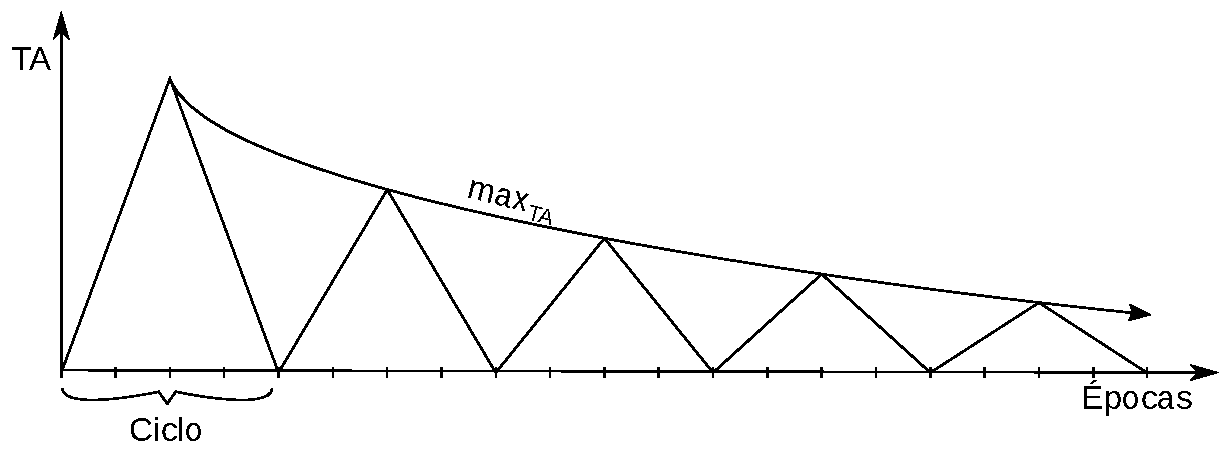
\includegraphics[width=0.7\textwidth]{./CLR.pdf}
	\caption{Esquema de la evolución de la tasa de aprendizaje durante las épocas de entrenamiento.}
	\label{fig:clr}
\end{figure}

Se utilizó un tamaño de lote de 24 imágenes, principalmente porque era la cantidad máxima que entraba en la memoria de
la GPU. Como función de pérdida se utilizó el \textit{likelihood} negativo logarítmico, dado que este es un problema de
clasificación multiclase. Como optimizador se utilizó gradiente descendiente estocástico (SGD, por sus siglas en inglés)
con una tasa de aprendizaje (TA) inicial de 0.0001 y un momento inicial de 0.9. Sin embargo, se utilizó un planificador
de TA cíclico \cite{smith2017cyclical}. Este aumenta la TA deforma lineal hasta un máximo de $max_{TA} = 0.1$ durante
dos épocas de entrenamiento (o lo que es lo mismo, 1024 lotes de entrenamiento) para luego reducir la TA de forma lineal
hasta el mínimo de 0.0001 a lo largo de dos épocas. Inversamente al TA, el momento es decrementado linealmente de su
valor base de $0.9$ hasta $0.5$ durante dos épocas para luego ser incrementado durante las dos épocas siguientes de
vuelta a su valor base. La proporción de cambio de ambos parámetros se va reduciendo levemente de forma exponencial con
un factor de $0.9$. Es decir, en el caso de la TA, durante el primer ciclo (4 épocas de entrenamiento) el $max_{TA}$ es
de $0.1$, durante el segundo ciclo es de $max_{TA}=0.9 \times 0.1=0.09$. A este esquema de entrenamiento se llego luego
de realizar varias pruebas con diferentes conjuntos de parámetros y comparando el error medio en validación cruzada.
Principalmente, la elección de SGD con planificador de TA cíclico resulto significativamente mejor que \textit{Adam} y
\textit{Adadelta}. Otro punto a resaltar es la magnitud de $max_{TA}$, que podría parecer demasiado elevada. Sin
embargo, las pruebas mostraban que valores inferiores hacían que los modelos se estanquen en mínimos locales y como
resultado alcancen menores tasas de aciertos en validación cruzada. Por otro lado, todos los parámetros de la red
excepto las dos capaz lineales (la que trae el modelo pre-entrenado y la anexada) se congelaban durante el primer ciclo
de entrenamiento. Como el modelo está pre-entrenado, se puede suponer que las primeras capaz convolucionales están
correctamente ajustadas. De hecho, ajustando sólo los pesos de las dos últimas capaz lineales se alcanzaba una tasa de
aciertos balanceada de $60\%$.

Finalmente, como se menciona en la introducción, es utilizó validación cruzada con 10 particiones. Para estimar la
cantidad óptima de épocas de entrenamiento se utilizó parada temprana, con 16 épocas de entrenamiento. Por lo general,
con 20 épocas de entrenamiento era suficiente para alcanzar el máximo en validación.

\bibliographystyle{abbrv}
\bibliography{bibliography}

\end{document}
